\FloatBarrier
\section{User-Controlled Walking}
\label{sec::41_uc}
As the fundamental building block for the comparison to autonomous walking, we now need to investigate on user-controlled walking. This enables us, in contrast to the control by a neural network, to find the best parameters for the pattern generation in a well controllable environment. These parameters will then be kept constant throughout the rest of this thesis, in order to allow for a good comparison between user-controlled walking and autonomously controlled walking. Furthermore, we will rely on them to gather data for the behavioral cloning approach in section \ref{sec::423_da}.
\FloatBarrier
\subsection{Benchmarking of Nonlinear Model Predictive Control}
\label{sec::411_bm}
To evaluate the pattern generator implementation of ours, we have benchmarked it against an existing one, which was written in Python. Therefore, we defined velocity commands, as they typically may appear in real-world scenarios. The four defined use cases, which are shown in figures \ref{fig::411_benchmarking_basic} and \ref{fig::411_benchmarking_advanced}, were parametrized in accordance to the HRP-2 humanoid robot.
\begin{figure}[h!]
	\centering
	\subcaptionbox{Straight trajectories at\\$\bm{v}=\begin{pmatrix}
		0.1 & 0.0 & 0.0
		\end{pmatrix}^T$.}%
	[.45\linewidth]{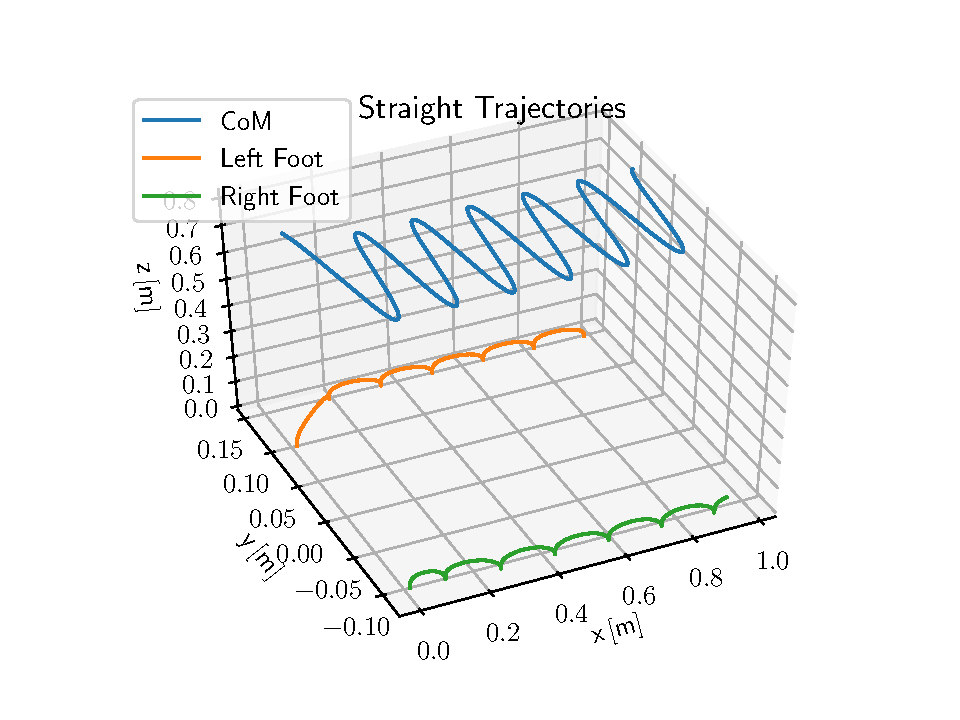
\includegraphics[scale=.45]{chapters/04_experiments/01_user_controlled_walking/01_benchmarking/nmpc_straight.pdf}}
	\subcaptionbox{Diagonal trajectories at\\$\bm{v}=\begin{pmatrix}
		0.1 & 0.1 & 0.0
		\end{pmatrix}^T$.}%
	[.45\linewidth]{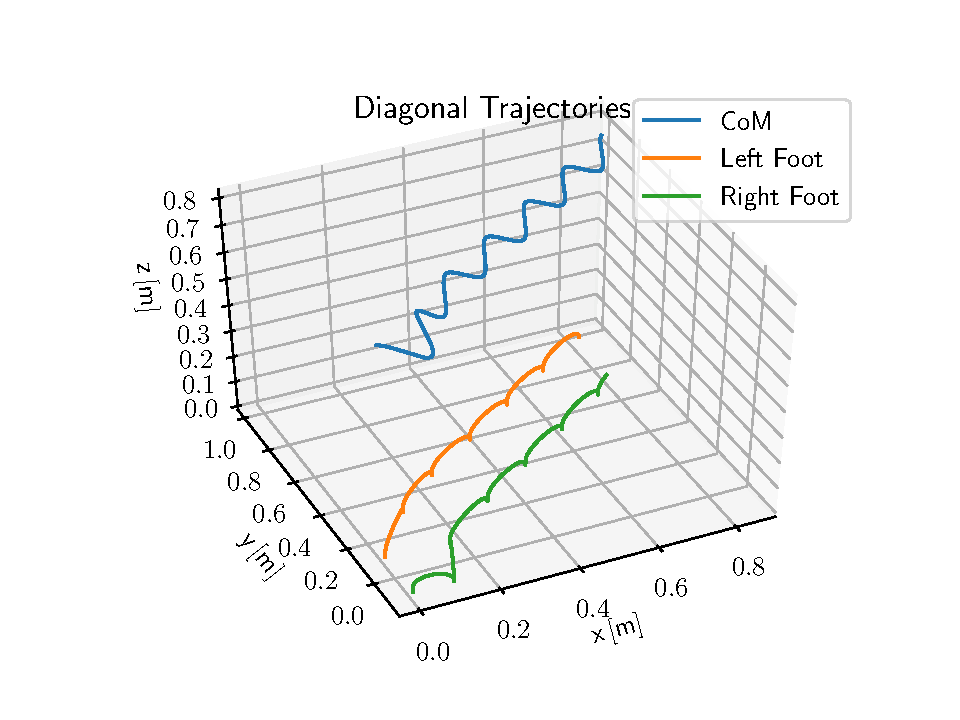
\includegraphics[scale=.45]{chapters/04_experiments/01_user_controlled_walking/01_benchmarking/nmpc_diagonal.pdf}}
	\caption{Simple trajectories. The velocities are given in units of\\$(\text{m}/\text{s}\,\,\,\,\text{m}/\text{s}\,\,\,\,\text{rad}/\text{s})^T$, where the first two entries describe the robot's velocity in the x-, and the y-direction, and the last entry describes the robot's angular velocity about the z-axis, form a frame that is attached to the robot. The trajectories start on the left-hand side.}
	\label{fig::411_benchmarking_basic}
\end{figure} 
The parameters for these tests can be found in the YAML file at the provided \href{https://github.com/mhubii/nmpc_pattern_generator/blob/719fde0bb73925923de85cbf379c5523e075dfeb/libs/pattern_generator/configs_hrp2.yaml#L1}{\underline{link}}. To obtain the pattern generator's performance, in terms of speed, the straight walk experiment in figure \ref{fig::411_benchmarking_basic} (a) got executed ten times on an Intel Core i7-7700HQ CPU at $2.8\,\text{GHz}$, for both, the Python and our implementation. It took $873\pm23\,\text{ms}$ and $147.7\pm0.5\,\text{ms}$ to execute the code for $100$ iterations on average, which means that a single iteration took $8.73\pm0.23\,\text{ms}$ and $1.48\pm0.01\,\text{ms}$. It was therefore possible to achieve a speed-up of around $600$ percent with the presented implementation. We further demonstrate the avoidance of a convex obstacle with a security margin that keeps the robot at a safe distance in figure \ref{fig::411_benchmarking_advanced} (b). The used obstacle is defined to be located at $x=1.6\,\text{m}$ and $y=1.0\,\text{m}$, with a radius of $R=1.0\,\text{m}$, and a security margin of $m=0.4\,\text{m}$.
\begin{figure}[h!]
	\centering
	\subcaptionbox{Curved trajectories at\\$\bm{v}=\begin{pmatrix}
	0.1 & 0.0 & 0.1
	\end{pmatrix}^T$.}%
	[.45\linewidth]{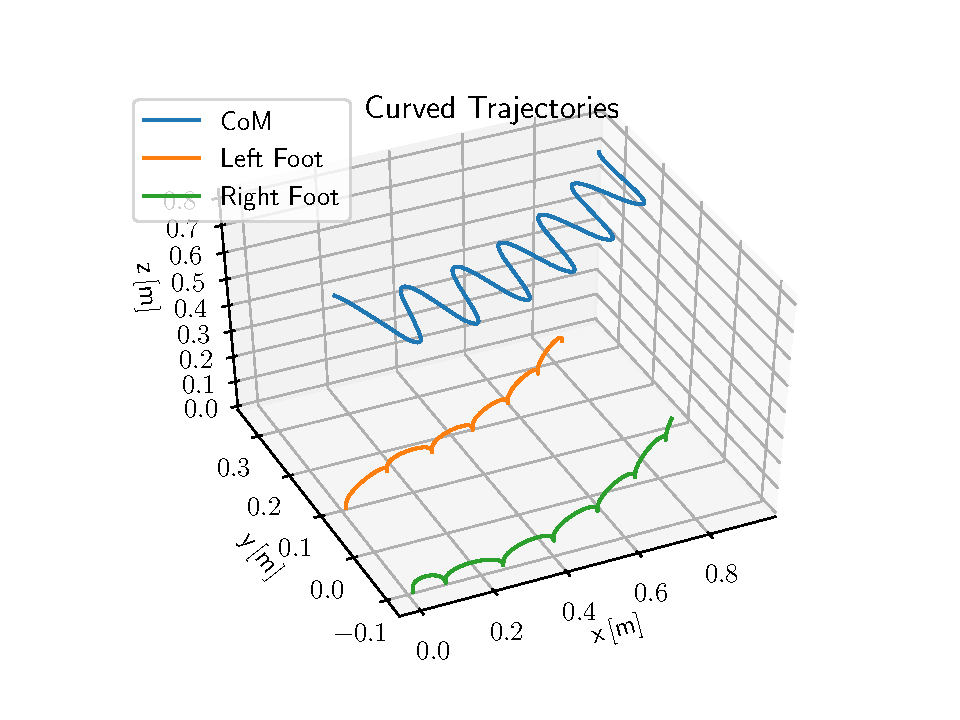
\includegraphics[scale=.45]{chapters/04_experiments/01_user_controlled_walking/01_benchmarking/nmpc_turn.pdf}}
	\subcaptionbox{Obstacle avoidance at\\$\bm{v}=\begin{pmatrix}
	0.1 & 0.0 & 0.0
	\end{pmatrix}^T$}%
	[.45\linewidth]{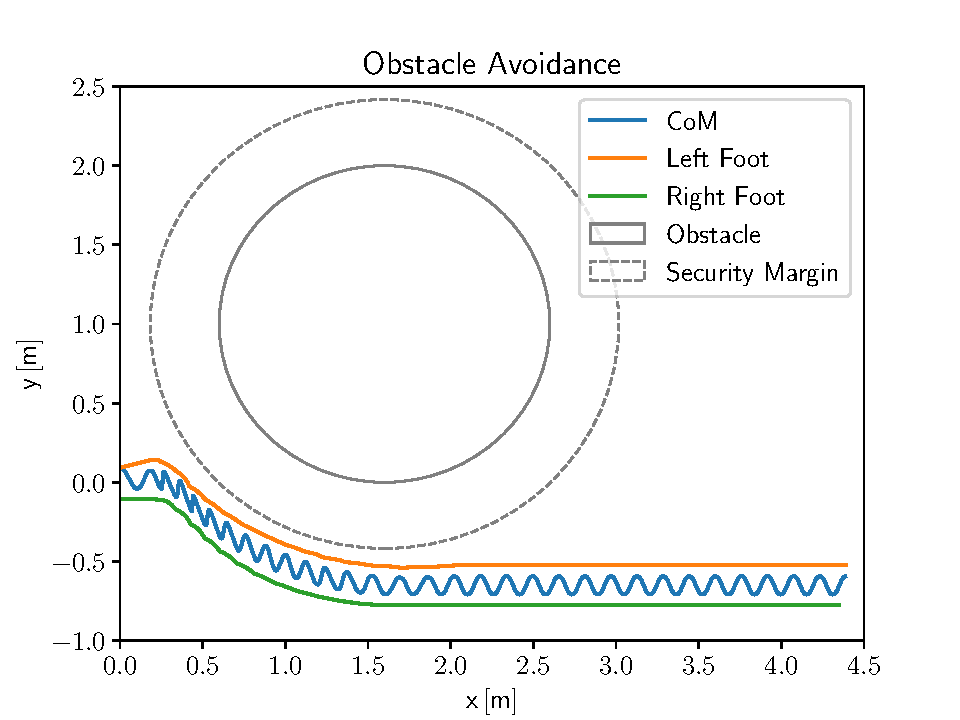
\includegraphics[scale=.45]{chapters/04_experiments/01_user_controlled_walking/01_benchmarking/nmpc_obstacle.pdf}}
	\caption{Advanced trajectories. The velocities are given in units of\\$(\text{m}/\text{s}\,\,\,\,\text{m}/\text{s}\,\,\,\,\text{rad}/\text{s})^T$, see figure \ref{fig::411_benchmarking_basic}.}
	\label{fig::411_benchmarking_advanced}
\end{figure} 
To always ensure a smooth motion, and to benchmark the interpolation, we plotted the x-, y-, and z-trajectories for the left and the right foot, as shown in figure \ref{fig::411_benchmarking_inter}. The plots were generated on the curved trajectory of figure \ref{fig::411_benchmarking_advanced} (a), and they reveal a continuous behavior at every time step for all dimensions.
\begin{figure}[h!]
	\centering
	\subcaptionbox{Interpolated\\x-Trajectories}%
	[.3\linewidth]{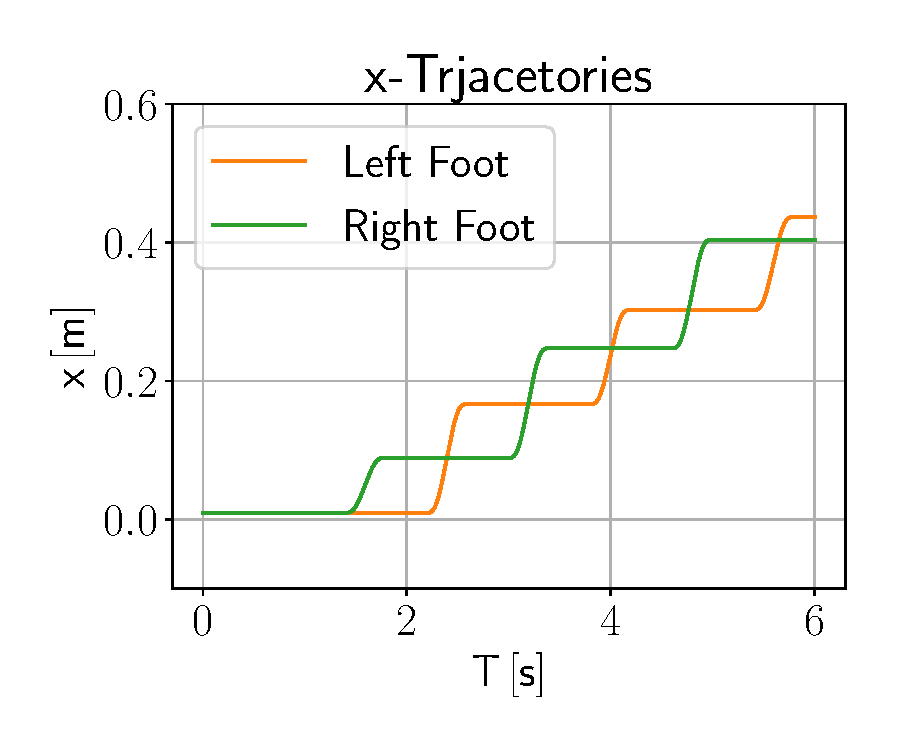
\includegraphics[scale=.3]{chapters/04_experiments/01_user_controlled_walking/01_benchmarking/interpolated_x_trajectories.pdf}}
	\subcaptionbox{Interpolated\\y-Trajectories}%
	[.3\linewidth]{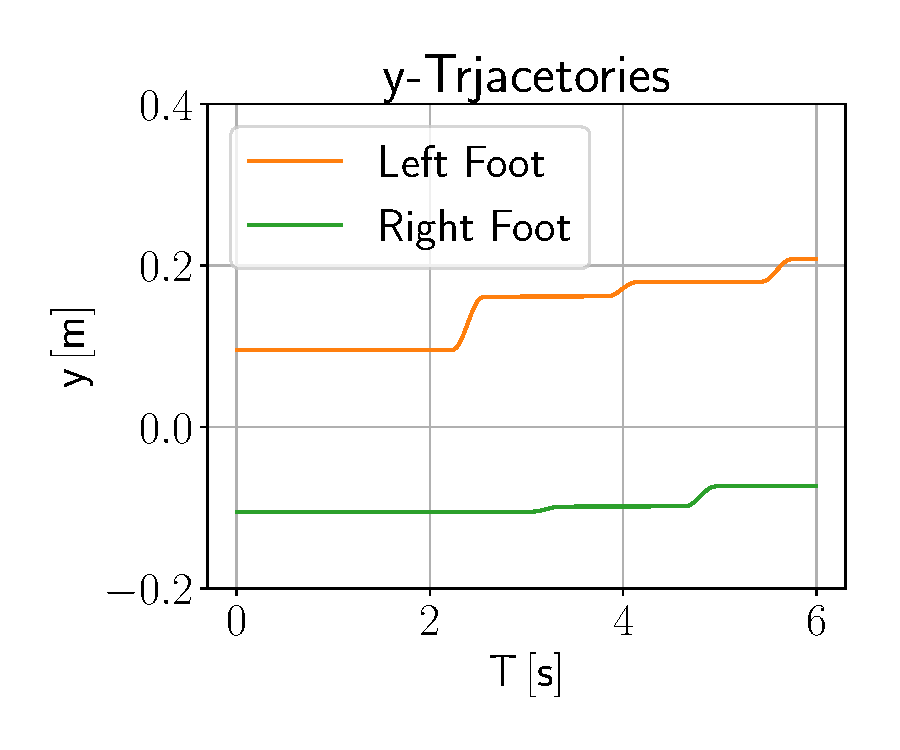
\includegraphics[scale=.3]{chapters/04_experiments/01_user_controlled_walking/01_benchmarking/interpolated_y_trajectories.pdf}}
	\subcaptionbox{Interpolated\\z-Trajectories}%
	[.3\linewidth]{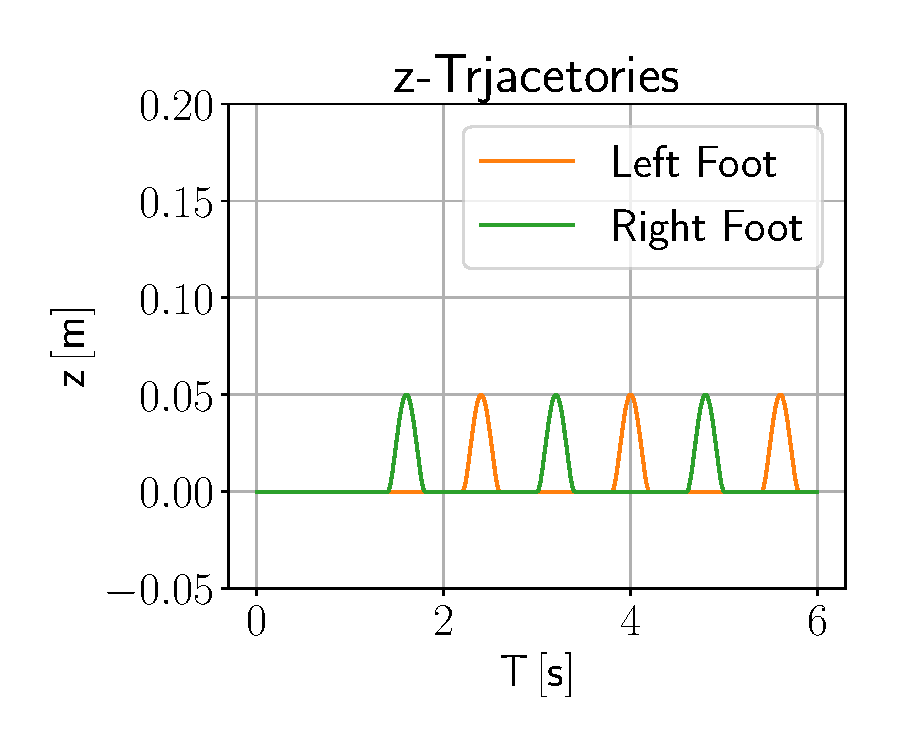
\includegraphics[scale=.3]{chapters/04_experiments/01_user_controlled_walking/01_benchmarking/interpolated_z_trajectories.pdf}}
	\caption{Interpolated foot trajectories. As explained in figure \ref{fig::213_ip}, the interpolation interpolates the feet's movement, given an initial, and a final foot position. The continuity shows that the interpolation got implemented correctly.}
	\label{fig::411_benchmarking_inter}
\end{figure}
 The benchmarked pattern generator then enabled us to run it on the real robot, which we did in a test environment that will be presented in the next section - Performance in Test Environment.
\FloatBarrier
\subsection{Performance in Test Environment}
\label{sec::412_pt}
For the execution on Heicub, we chose a parameter setting with which we could ensure balanced motion for all velocity commands. This could be achieved by choosing the parameters, which are listed in the YAML configurations file at the provided \href{https://github.com/mhubii/nmpc_pattern_generator/blob/719fde0bb73925923de85cbf379c5523e075dfeb/libs/pattern_generator/configs.yaml#L1}{\underline{link}}. The most important ones therein are further shown in table \ref{tab::412_params}.
\begin{table}
	\centering
	\caption{Parameters which used to work best on Heicub.}
	\begin{tabular}{lclc}
		Parameter&Value&Parameter&Value\\
		\hline
		$T_{\text{Step}}$ & $3.20\,\text{s}$ & $N$ & $16\,\text{\#}$ \\
		$T_{\text{Double Support}}$ & $1.60\,\text{s}$ & $\alpha$ & $1.0\,\text{a.u.}$ \\
		$T_{\text{Command Period}}$  & $0.01\,\text{s}$& $\beta$ & $100\,\text{a.u.}$ \\
		$T_{\text{Preview}}$ & $0.40\,\text{s}$ & $\gamma$ & $0.01\,\text{a.u.}$
	\end{tabular}
	\label{tab::412_params}
\end{table}
Now given these parameters, we designed an environment for Heicub to walk in. A human user had to control the robot in four different scenarios. In each of the scenarios, Heicub started from a reference position, in order to reach a fire extinguisher at a distant location. By design, the setup allows for benchmarking of dynamic balance in all four different scenarios. As will be shown in section \ref{sec::42_ab}, we require a neural network to execute the same tasks, and therefore we can compare the performances of a human user with that of an autonomous agent. For the dynamic balance evaluation, we extracted the desired ZMP from the nonlinear model predictive controller, and measured the true ZMP, in accordance to equations \ref{eq::211_double_zmp_x} and \ref{eq::211_double_zmp_y}, by recording the ankles' force-torque sensor readouts. We further kept track of the velocity commands to the pattern generator for all tasks to extract the user's behavior. The first task was simply to go two meters straight forward (figure \ref{fig::412_uc_straight}).
\begin{figure}[h!]
	\subcaptionbox{Dynamic balance.}%
	[.5\linewidth]{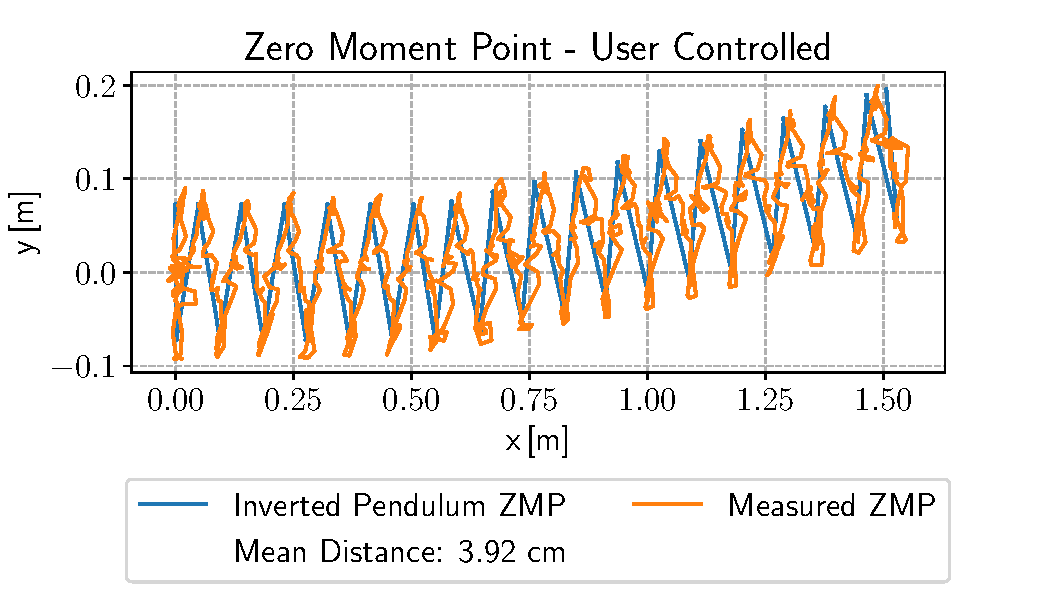
\includegraphics[scale=.45]{chapters/04_experiments/01_user_controlled_walking/02_test_environment/straight_walk_01_zmp.pdf}}
	\subcaptionbox{Behavior.}%
	[.5\linewidth]{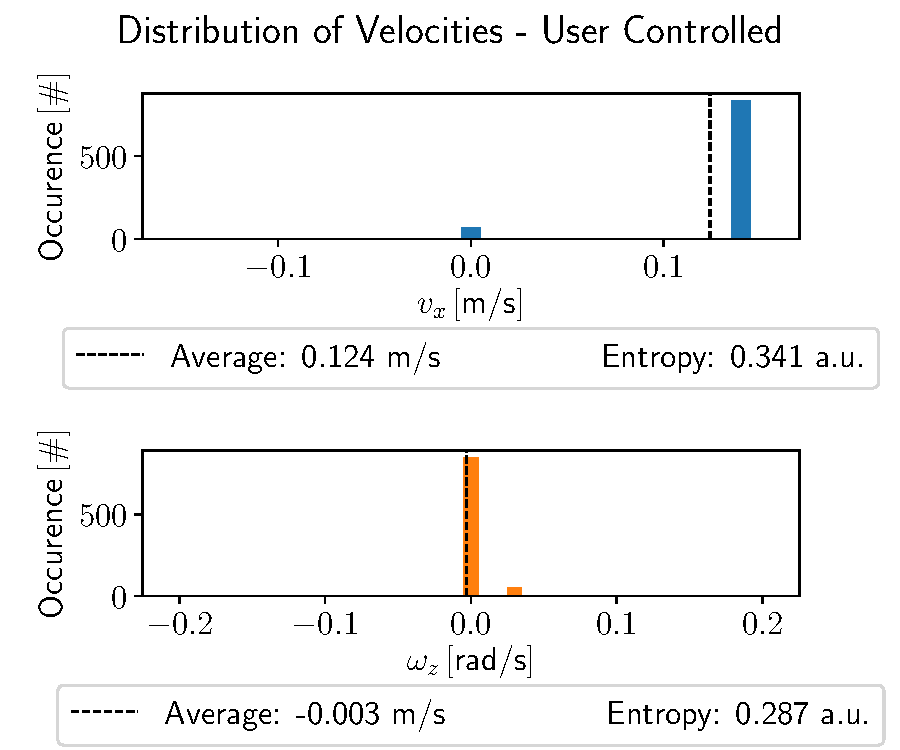
\includegraphics[scale=.45]{chapters/04_experiments/01_user_controlled_walking/02_test_environment/straight_walk_01_entropy.pdf}}
	\caption{User-controlled straight walk. The robot started to the plot's left-hand side (a), and moved forward until it reached the fire extinguisher.}
	\label{fig::412_uc_straight}
\end{figure} 
The behavior therein is visualized by a histogram of all velocity commands over the course of the task (figure \ref{fig::412_uc_straight} (b)). For the bin size we chose $0.01\,\text{m}/\text{s}$ and $0.01\,\text{rad}/\text{s}$, respectively. 
\begin{figure}[h!]
	\subcaptionbox{Dynamic balance.}%
	[.5\linewidth]{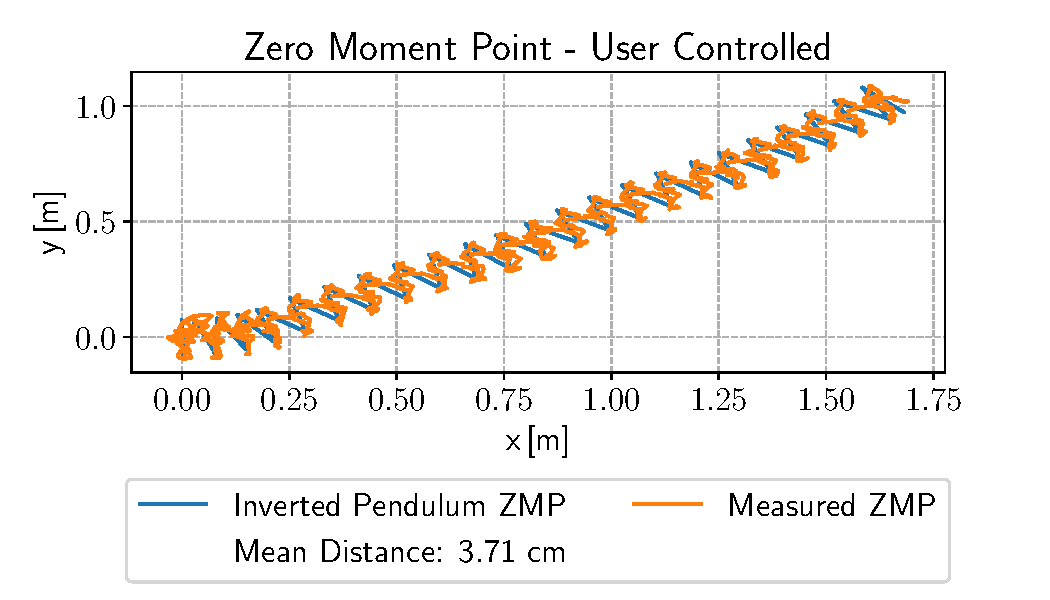
\includegraphics[scale=.45]{chapters/04_experiments/01_user_controlled_walking/02_test_environment/curved_walk_01_zmp.pdf}}
	\subcaptionbox{Behavior.}%
	[.5\linewidth]{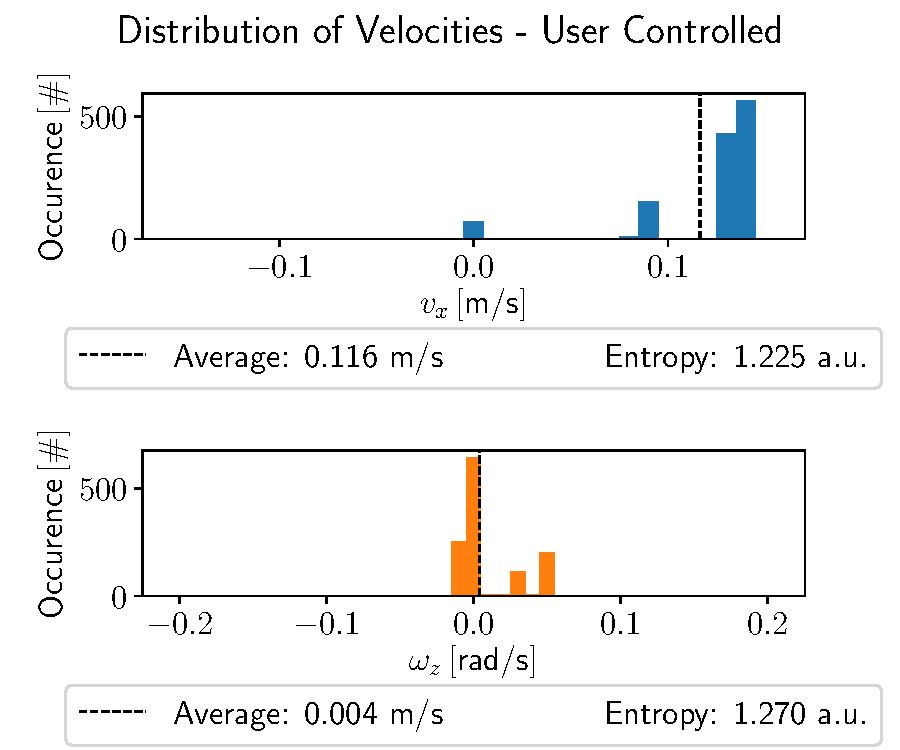
\includegraphics[scale=.45]{chapters/04_experiments/01_user_controlled_walking/02_test_environment/curved_walk_01_entropy.pdf}}
	\caption{User-controlled curved walk. The robot started to the plot's left-hand side (a), and performed a left turn on its way to the fire extinguisher, where it stopped.}
	\label{fig::412_uc_curved}
\end{figure} 
The second task was to reach the fire extinguisher, which was located to the left of the robot. In order to reach it, it was therefore required to perform a curved walk (figure \ref{fig::412_uc_curved}). The third task (figure \ref{fig::412_uc_obstacle}) involved the avoidance of an obstacle, namely a chair. For the fourth task (figure \ref{fig::412_uc_sight}), the robot started with its back pointing towards the fire extinguisher.
\begin{figure}[h!]
	\subcaptionbox{Dynamic balance.}%
	[.5\linewidth]{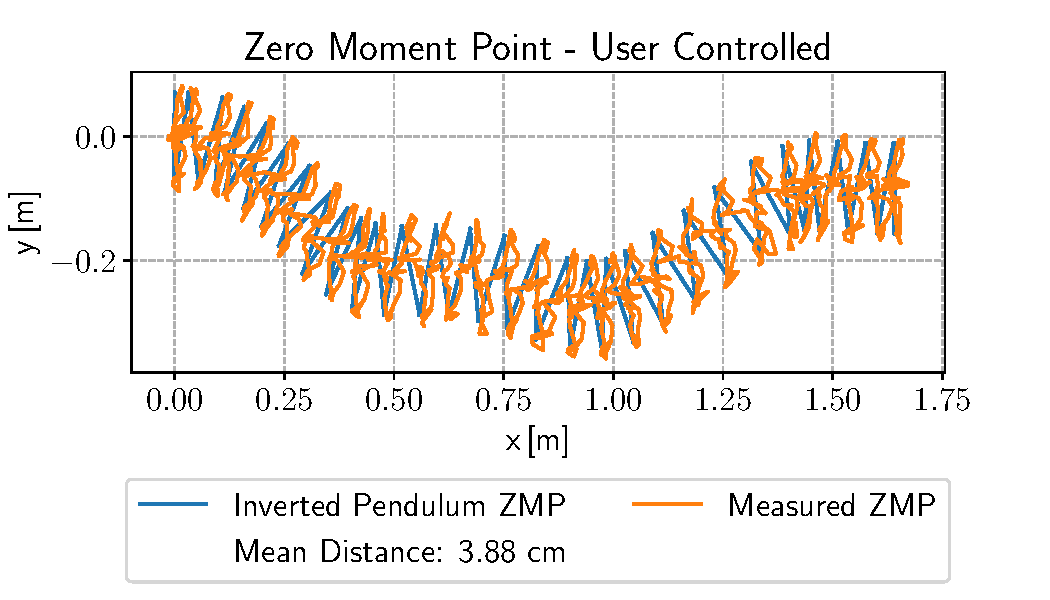
\includegraphics[scale=.45]{chapters/04_experiments/01_user_controlled_walking/02_test_environment/obstacle_walk_02_zmp.pdf}}
	\subcaptionbox{Behavior.}%
	[.5\linewidth]{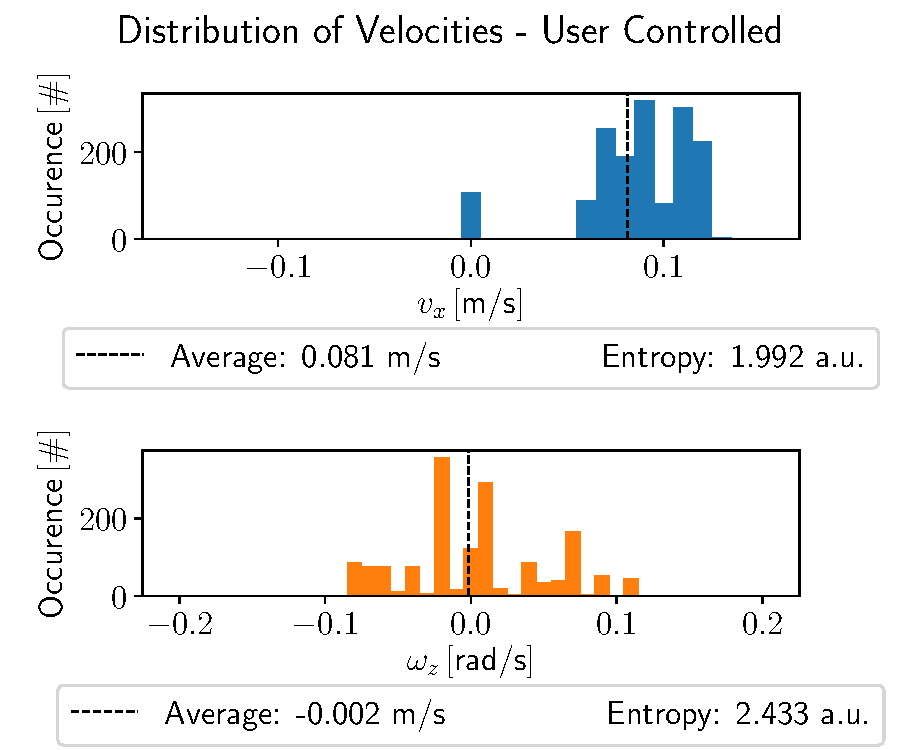
\includegraphics[scale=.45]{chapters/04_experiments/01_user_controlled_walking/02_test_environment/obstacle_walk_02_entropy.pdf}}
	\caption{User-controlled obstacle avoidance. The robot started to the plot's left-hand side (a), and moved towards a fire extinguisher. On about half of the distance it avoided a chair by turning to the right, and then to the left again, until it reached the fire extinguisher and stopped.}
	\label{fig::412_uc_obstacle}
\end{figure} 
\begin{figure}[h!]
	\subcaptionbox{Dynamic balance.}%
	[.5\linewidth]{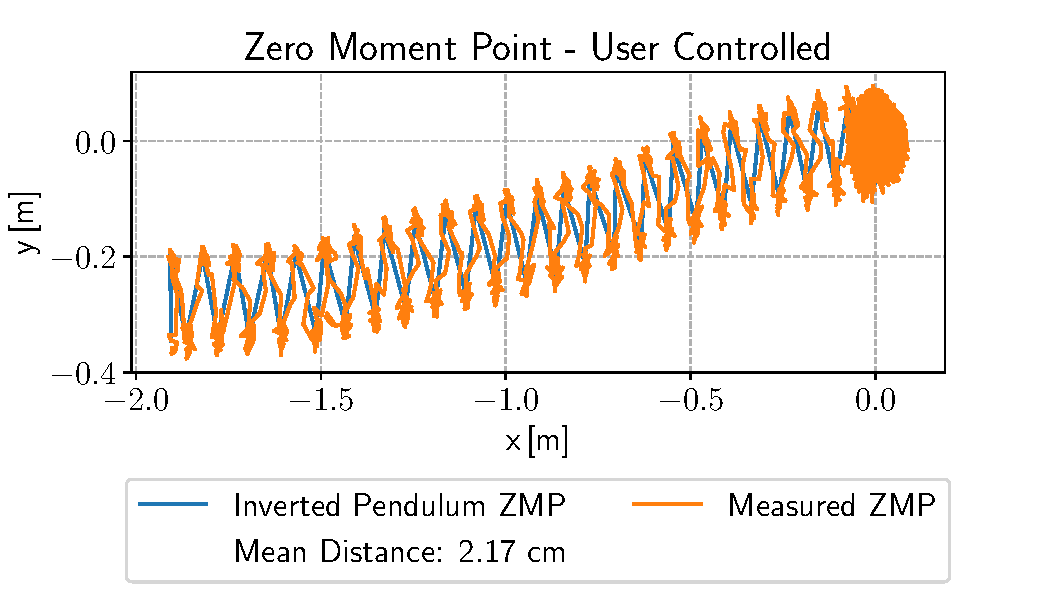
\includegraphics[scale=.45]{chapters/04_experiments/01_user_controlled_walking/02_test_environment/out_of_sight_walk_01_zmp.pdf}}
	\subcaptionbox{Behavior.}%
	[.5\linewidth]{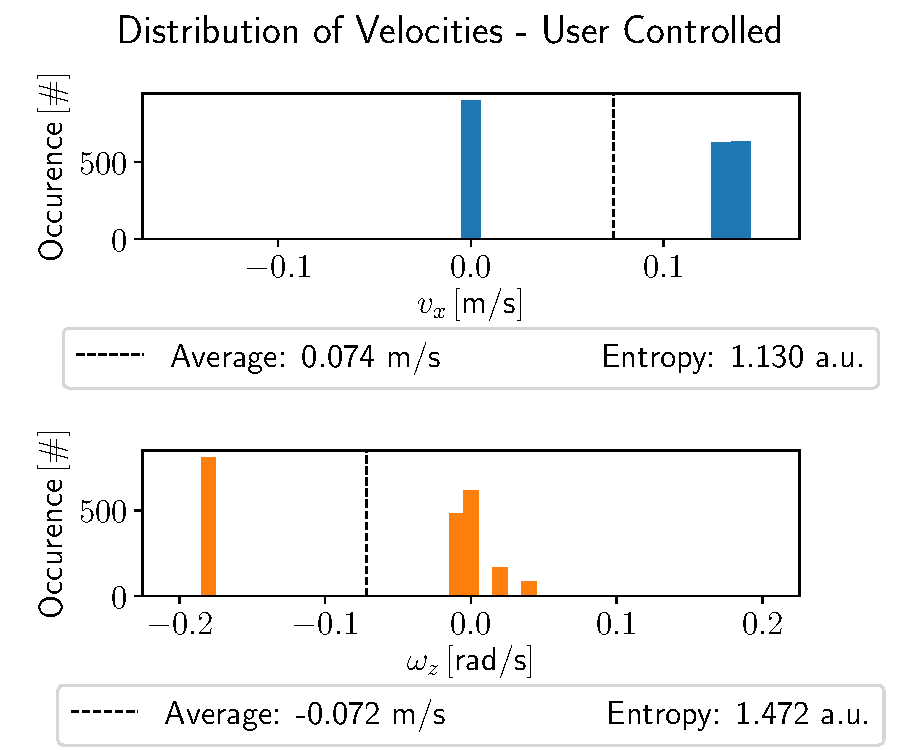
\includegraphics[scale=.45]{chapters/04_experiments/01_user_controlled_walking/02_test_environment/out_of_sight_walk_01_entropy.pdf}}
	\caption{User-controlled environmental scanning. The robot started to the plot's right-hand side (a), facing to the right, and performed a full $180^\circ$ turn, before walking almost straight to the fire extinguisher, which is here located to the plot's left-hand side.}
	\label{fig::412_uc_sight}
\end{figure} 
\newpage